\documentclass[10pt,letterpaper]{article}

\usepackage[margin=0.84in,top=0.86in,bottom=0.86in,headheight=14pt,headsep=14pt]{geometry}
\usepackage{amsmath,amssymb,amsthm,mathtools}
\usepackage{fontspec}
\usepackage{microtype}
\usepackage{booktabs}
\usepackage{array}
\usepackage{float}
\usepackage{graphicx}
\usepackage{xcolor}
\usepackage{enumitem}
\usepackage{fancyhdr}
\usepackage[most]{tcolorbox}
\usepackage{listings}
\usepackage[colorlinks=true,linkcolor=accentblue,citecolor=accentblue,urlcolor=accentblue,
  pdftitle={No Finite-Dimensional Extremizer for Subquadratic Lee Constants (MI-20)},
  pdfauthor={Marcio Diaz (Space AI)},
  pdfsubject={Open Problem MI-20 (OpenProblemsInNLA), Matrix Analysis, Schatten Norms},
  pdfkeywords={Lee conjecture, Schatten norms, MI-20, Space AI, Marcio Diaz}]{hyperref}

% Fonts (Tectonic / XeTeX bundled TeX Gyre Pagella + Heros + Cursor)
\setmainfont{texgyrepagella}[
  Extension=.otf,
  UprightFont=*-regular,
  BoldFont=*-bold,
  ItalicFont=*-italic,
  BoldItalicFont=*-bolditalic
]
\setsansfont{texgyreheros}[
  Extension=.otf,
  UprightFont=*-regular,
  BoldFont=*-bold,
  ItalicFont=*-italic,
  BoldItalicFont=*-bolditalic,
  Scale=MatchLowercase
]
\setmonofont{texgyrecursor}[
  Extension=.otf,
  UprightFont=*-regular,
  BoldFont=*-bold,
  ItalicFont=*-italic,
  BoldItalicFont=*-bolditalic,
  Scale=0.86
]

% Color palette
\definecolor{ink}{HTML}{0F2537}
\definecolor{accentblue}{HTML}{1D4ED8}
\definecolor{accentteal}{HTML}{0F766E}
\definecolor{muted}{HTML}{52606D}
\definecolor{boxbg}{HTML}{F4F8FC}
\definecolor{boxborder}{HTML}{2563EB}
\definecolor{statusbg}{HTML}{FFFBEB}
\definecolor{statusborder}{HTML}{D97706}
\definecolor{remarkbg}{HTML}{F8FAFC}
\definecolor{remarkborder}{HTML}{64748B}
\definecolor{codebg}{HTML}{0F172A}
\definecolor{codefg}{HTML}{E2E8F0}

\linespread{1.04}
\setlength{\parskip}{3.8pt}
\setlength{\parindent}{0pt}
\setlength{\emergencystretch}{2.5em}
\allowdisplaybreaks[2]

% Running header/footer
\pagestyle{fancy}
\fancyhf{}
\fancyhead[L]{\sffamily\footnotesize\itshape\color{muted}No Finite-Dimensional Extremizer for Subquadratic Lee Constants (MI-20)}
\fancyhead[R]{\sffamily\footnotesize\color{muted}\thepage}
\renewcommand{\headrulewidth}{0.4pt}
\renewcommand{\headrule}{\hbox to\headwidth{\color{muted!40}\leaders\hrule height \headrulewidth\hfill}}

\fancypagestyle{firstpage}{
  \fancyhf{}
  \fancyfoot[C]{\sffamily\footnotesize\color{muted}\thepage}
  \renewcommand{\headrulewidth}{0pt}
}

% Section formatting
\usepackage{titlesec}
\titleformat{\section}{\sffamily\bfseries\large\color{ink}}{\thesection.}{0.5em}{}
\titlespacing*{\section}{0pt}{14pt}{5pt}
\titleformat{\subsection}{\sffamily\bfseries\normalsize\color{ink}}{\thesubsection}{0.5em}{}
\titlespacing*{\subsection}{0pt}{10pt}{3pt}

% Framed theorem / lemma / status boxes
\tcbset{
  mathbox/.style={
    enhanced,
    colback=boxbg, colframe=boxborder!55,
    boxrule=0.5pt, leftrule=3pt, arc=2pt,
    top=5.5pt, bottom=5.5pt, left=8.5pt, right=8.5pt,
    before skip=7pt, after skip=7pt
  },
  lemmabox/.style={
    enhanced,
    colback=remarkbg, colframe=ink!35,
    boxrule=0.5pt, leftrule=2.5pt, arc=2pt,
    top=5pt, bottom=5pt, left=8pt, right=8pt,
    before skip=6.5pt, after skip=6.5pt
  },
  statusbox/.style={
    enhanced,
    colback=statusbg, colframe=statusborder!75,
    boxrule=0.6pt, leftrule=3pt, arc=2pt,
    top=5.5pt, bottom=5.5pt, left=8.5pt, right=8.5pt,
    before skip=6pt, after skip=6pt
  },
  abstractbox/.style={
    enhanced,
    colback=boxbg!85, colframe=boxborder!45,
    boxrule=0.5pt, leftrule=3pt, arc=2pt,
    top=6pt, bottom=6pt, left=9pt, right=9pt,
    before skip=6pt, after skip=6pt
  },
  codebox/.style={
    enhanced,
    colback=codebg, colframe=codebg,
    boxrule=0pt, arc=3pt,
    top=6pt, bottom=6pt, left=8pt, right=8pt,
    before skip=6pt, after skip=5pt
  }
}

% Code listing style (rendered cleanly inside codebox with zero hairline artifacts)
\lstset{
  language=Python,
  basicstyle=\ttfamily\footnotesize\color{codefg},
  keywordstyle=\color{cyan!65}\bfseries,
  commentstyle=\color{gray!70}\itshape,
  stringstyle=\color{lime!75},
  frame=none,
  aboveskip=0pt, belowskip=0pt,
  breaklines=true,
  showstringspaces=false
}

% Math macros
\newcommand{\C}{\mathbb{C}}
\newcommand{\R}{\mathbb{R}}
\newcommand{\Hilb}{\mathcal{H}}
\newcommand{\Sp}{\mathcal{S}_p}
\newcommand{\Tr}{\operatorname{Tr}}
\newcommand{\ran}{\operatorname{ran}}
\newcommand{\rank}{\operatorname{rank}}
\newcommand{\diag}{\operatorname{diag}}
\newcommand{\op}{\mathrm{op}}
\newcommand{\TZ}{\mathrm{TZ}}
\newcommand{\conc}{\mathrm{conc}}
\newcommand{\lin}{\mathrm{lin}}
\newcommand{\abs}[1]{\lvert #1 \rvert}
\newcommand{\norm}[1]{\lVert #1 \rVert}

\begin{document}
\thispagestyle{firstpage}

% Top institutional/classification banner
{\sffamily\footnotesize\bfseries\color{accentblue}MATHEMATICAL WHITEPAPER $\cdot$ MATRIX ANALYSIS \hfill OPEN PROBLEM MI-20 (OPENPROBLEMSINNLA)}\par
\vspace{2pt}
{\color{ink}\hrule height 1.1pt}
\vspace{12pt}

\begin{center}
  {\LARGE\bfseries\color{ink} No Finite-Dimensional Extremizer for Subquadratic\\[3pt] Lee Constants}\par
  \vspace{7pt}
  {\large\itshape\color{muted} Strict Infinite-Dimensional Hierarchy, Universal $2\times 2$ Collapse, Exact Algebraic\\[1pt] Evaluations, and Zero-Float Rational Certificates for Problem MI-20}\par
  \vspace{9pt}
  {\normalsize\bfseries Marcio Diaz}\textsuperscript{1}\par
  {\small\color{muted}\textsuperscript{1}Space AI (\href{https://spaceresearch.ai}{spaceresearch.ai}) \quad $\cdot$ \quad November 27, 2026 \quad $\cdot$ \quad MSC 2020: 15A60, 47A30, 47B10, 15A45}
\end{center}
\vspace{4pt}

\begin{tcolorbox}[abstractbox]
{\sffamily\footnotesize\bfseries\color{accentblue}ABSTRACT}\par\vspace{2pt}
For a Schatten exponent $p \ge 1$ and $m \ge 2$ matrices, Eun-Young Lee's quasi-reverse Minkowski problem asks for the optimal dimension-independent constant $C_{p,m}$ in
\[
  \Bigl\|\sum_{k=1}^m A_k\Bigr\|_p \le C_{p,m}\,\Bigl\|\sum_{k=1}^m |A_k|\Bigr\|_p,
  \qquad |X| := (X^* X)^{1/2}.
\]
For $p = 1$ the optimal constant $C_{1,m} = 1$ is attained in dimension $n = 1$, and for every $p \ge 2$ Hongsen Qiu (August 2026) proved that $C_{p,m}$ is attained in finite dimension $n = m$ by equiangular rank-one matrices. By contrast, determining $C_{p,m}$ in the subquadratic range $1 < p < 2$ remains open as Problem~\textbf{MI-20} in \emph{Open Problems in Numerical Linear Algebra}.

We prove a sharp dimensional phase transition at $p = 2$: for every $1 < p < 2$ and every $m \ge 2$, the finite-dimensional optimal constants form a \textbf{strictly increasing infinite sequence}
\[
  1 = C_{p,m}(1) < C_{p,m}(2) < C_{p,m}(3) < \cdots < C_{p,m}(n) < C_{p,m}(n+1) < \cdots < C_{p,m}(\infty)
\]
over both $\C$ and $\R$, confirming unconditionally a conjecture of Qiu (2026). Via Xing Li's concave-function transfer theorem (2026), the same strict infinite hierarchy holds for Lee's nonlinear concave-function Schatten constants. Even on an infinite-dimensional separable Hilbert space $\Hilb$, no tuple in $(\Sp(\Hilb))^m$ containing even a single finite-rank operator can attain $C_{p,m}(\infty)$. The proof is completely self-contained and elementary, combining polar optimality, an isometric left-rotation perturbation, universal rank deficiency of finite maximizers, and a sharp Sherman--Morrison rank-one Schatten-$p$ upper smoothness bound; we also prove the complementary superquadratic obstruction that for every $p \ge 2$, every finite-dimensional maximizer must have $\rank(S) < \rank(H)$.

In dimension $n = 2$, a short positive-duality Cauchy--Schwarz argument establishes a \textbf{universal $2\times 2$ collapse}: $C_{p,m}(2) = C_{p,m}^{\R}(2) = C_{p,2}(2)$ for \emph{every} $m \ge 2$ and \emph{every} $p > 1$, with exact algebraic evaluations $C_{3/2,m}(2) = \bigl(\frac{107+51\sqrt{17}}{256}\bigr)^{1/6} \approx 1.036414357333$ and a monic cubic characterization at $p = 4/3$ giving $C_{4/3,m}(2) \approx 1.018302375431$. Finally, explicit small-integer $2\times 3$ pairs at $p \in \{3/2, 4/3, 5/4\}$ strictly surpass $C_{p,m}(2)$ and are certified without floating-point arithmetic using pure Python integer/rational interval certificates.
\end{tcolorbox}

\begin{tcolorbox}[statusbox]
{\sffamily\footnotesize\bfseries\color{statusborder!90!black}SCOPE AND PROBLEM STATUS (MI-20 REMAINS OPEN)}\par\vspace{1.5pt}
{\small This whitepaper establishes a \textbf{structural partial resolution} of Problem~\textbf{MI-20}: Theorems~1--4 completely settle finite-dimensional and finite-rank non-attainment for every $1 < p < 2$ and $m \ge 2$, determine the exact $2\times 2$ constant for all $m \ge 2$ and $p > 1$, and certify explicit small-integer witnesses surpassing the $2\times 2$ barrier. Problem~\textbf{MI-20} itself asks to determine the exact value of $C_p(m) = C_{p,m}(\infty)$ as an explicit function of $(p,m)$ and therefore \textbf{remains Open}. All proofs have undergone line-by-line independent AI-assisted audit alongside exact zero-float rational and symbolic verification; no formal proof-assistant (Lean) verification or external human peer review has yet been performed.}
\end{tcolorbox}

\section{Introduction and Background}

For complex scalars $a_1,\dots,a_m$, the triangle inequality $|\sum_{k=1}^m a_k| \le \sum_{k=1}^m |a_k|$ holds with constant~$1$. In matrix analysis, the noncommutative analogue comparing the sum $S = \sum_{k=1}^m A_k$ against the sum of polar moduli $H = \sum_{k=1}^m |A_k|$ fails with constant~$1$ for every Schatten $p$-norm with $p > 1$. This led Eun-Young Lee~\cite{Lee2010,Lee2011} in 2010 to ask for the optimal dimension-independent constants $C_{p,m}$ satisfying
\begin{equation}\label{eq:lee}
  \Bigl\|\sum_{k=1}^m A_k\Bigr\|_p \le C_{p,m}\,\Bigl\|\sum_{k=1}^m |A_k|\Bigr\|_p,
\end{equation}
where $\|X\|_p := \bigl(\Tr(|X|^p)\bigr)^{1/p}$ denotes the Schatten $p$-norm and $|X| := (X^* X)^{1/2}$.

Lee conjectured for the Frobenius norm ($p = 2, m = 2$) that $C_{2,2} = \sqrt{\frac{1+\sqrt{2}}{2}} \approx 1.098684$, attained by two $2\times 2$ rank-one matrices; this was proved by Lin and Zhang~\cite{LinZhang2022} in 2022. Tang and Zhang~\cite{TangZhang2026} extended the Frobenius theorem to arbitrary $m \ge 2$ ($C_{2,m} = \sqrt{(1+\sqrt{m})/2}$) and conjectured a closed-form constant for all $p > 1$ derived from equiangular rank-one matrices sharing a left singular vector:
\begin{equation}\label{eq:tz}
  C_{p,m}^{\TZ} = \frac{\sqrt{x(x + m - 1)}}{(x^p + m - 1)^{1/p}},
  \qquad \text{where } x^p = 2x + m - 1,\quad x > 1.
\end{equation}

In August 2026, Hongsen Qiu~\cite{Qiu2026} proved unconditionally that $C_{p,m} = C_{p,m}^{\TZ}$ holds for every $p \ge 2$ and every $m \ge 2$ across all finite dimensions—confirming in particular that the optimal constant stabilizes at finite dimension $n = m$ (and at $n = 2$ for two matrices). Concurrently, Zeng, Liu, and Ratnavelu~\cite{Zeng2026} disproved~\eqref{eq:tz} at $p = 3/2$ via an exact rational $2\times 2$ rank-one counterexample, while Qiu~\cite{Qiu2026} systematically disproved~\eqref{eq:tz} for every subquadratic exponent $1 < p < 2$ using a two-parameter family $F_p(c,d)$ of equal-norm rank-one pairs. Crucially, Qiu~\cite[\S5]{Qiu2026} also observed a floating-point $3\times 3$ pair at $p = 6/5$ slightly exceeding $\max_{c,d} F_{6/5}(c,d)$ and speculated that for $1 < p < 2$ the sharp constant might not be attained in any fixed dimension and may grow strictly with ambient dimension.

Shortly thereafter, Xing Li~\cite{Li2026} proved that the sharp constant in~\eqref{eq:lee} transfers without loss to arbitrary nonnegative concave functions applied to $|S|$ and $|A_k|$ in every fixed dimension $n$, and highlighted determining the subquadratic constants for $1 < p < 2$ as Problem~4.2—now cataloged as \textbf{Problem MI-20} in \emph{Open Problems in Numerical Linear Algebra}~\cite{OpenProblemsNLA}. In September 2026, Sidney Holden~\cite{Holden2026} contributed reviewed partial results on MI-20, including a positive power-system characterization, interpolation bounds, and the certified two-summand enclosure $1.018371575 < C_{4/3,2}(\infty) \le (861/800)^{1/4} \approx 1.018540473$.

\medskip
\textbf{Main discoveries of this paper.}
We prove that the dimensional phase transition at $p = 2$ is completely sharp and universal: for \emph{every} $1 < p < 2$ and \emph{every} $m \ge 2$, \emph{every finite-dimensional ansatz is strictly suboptimal}, and even in infinite-dimensional Hilbert spaces $\Sp(\Hilb)$ no tuple containing even one finite-rank operator can attain $C_{p,m}(\infty)$. Conversely, we show structurally why $p \ge 2$ behaves differently: our kernel-lifting lemma extends to $p \ge 2$ and forces $\rank(S) < \rank(H)$ at every superquadratic maximizer, whereas for $1 < p < 2$ isometric left-rotation forbids $\ker(S) \cap \ran(H) \neq \{0\}$. In addition, we establish a short universal $2\times 2$ collapse theorem ($C_{p,m}(2) = C_{p,2}(2)$ for all $m \ge 2$ and $p > 1$), derive exact algebraic characterizations at $p = 3/2$ and $p = 4/3$, and provide zero-float exact rational certificates for explicit $2\times 3$ integer witnesses at $p \in \{3/2, 4/3, 5/4\}$.

\section{Statement of Main Results}

For integers $n \ge 1$ and $m \ge 2$ and real $p > 1$, define the $n$-dimensional complex and real Lee constants by
\begin{equation}\label{eq:defC}
  C_{p,m}(n) := \sup_{A_1,\dots,A_m \in \C^{n\times n}} \frac{\|A_1 + \cdots + A_m\|_p}{\||A_1| + \cdots + |A_m|\|_p},
  \qquad
  C_{p,m}^{\R}(n) := \sup_{A_1,\dots,A_m \in \R^{n\times n}} \frac{\|A_1 + \cdots + A_m\|_p}{\||A_1| + \cdots + |A_m|\|_p},
\end{equation}
where the suprema are taken over nonzero tuples, and set $C_{p,m}(\infty) := \sup_{n \ge 1} C_{p,m}(n)$ and $C_{p,m}^{\R}(\infty) := \sup_{n \ge 1} C_{p,m}^{\R}(n)$. Throughout, let $p' := \frac{p}{p-1}$, $S := \sum_{k=1}^m A_k$, $H := \sum_{k=1}^m |A_k|$, and for a singular value decomposition $S = U_S \Sigma_S V_S^*$ define the dual operator $G_S := U_S \Sigma_S^{p-1} V_S^*$ (with $0^{p-1} := 0$).

\begin{tcolorbox}[mathbox]
\textbf{Theorem 1 (Strict Infinite-Dimensional Hierarchy for MI-20).}
\emph{For every $1 < p < 2$, every $m \ge 2$, and every integer $n \ge 1$,}
\[
  1 = C_{p,m}(1) < C_{p,m}(2) < C_{p,m}(3) < \cdots < C_{p,m}(n) < C_{p,m}(n+1) < \cdots < C_{p,m}(\infty),
\]
\emph{and identically over real matrices:}
\[
  1 = C_{p,m}^{\R}(1) < C_{p,m}^{\R}(2) < C_{p,m}^{\R}(3) < \cdots < C_{p,m}^{\R}(n) < C_{p,m}^{\R}(n+1) < \cdots < C_{p,m}^{\R}(\infty).
\]
\emph{In particular, no finite-dimensional matrix tuple attains the sharp subquadratic Lee constant.}
\end{tcolorbox}

Combining Theorem~1 with Xing Li's fixed-dimension concave-function transfer theorem~\cite[Theorem~1.1]{Li2026} yields an immediate nonlinear consequence.

\begin{tcolorbox}[lemmabox]
\textbf{Corollary 1 (Strict Hierarchy for Concave-Function Lee Constants).}
\emph{For every $1 < p < 2$ and $m \ge 2$, let $c_{p,m,n}^{\conc}$ be the optimal constant in $\|f(|\sum_{k=1}^m A_k|)\|_p \le c_{p,m,n}^{\conc} \|\sum_{k=1}^m f(|A_k|)\|_p$ over all $A_1,\dots,A_m \in \C^{n\times n}$ and all nonnegative concave functions $f : [0,\infty) \to [0,\infty)$. Because $c_{p,m,n}^{\conc} = C_{p,m}(n)$ for every finite $n \ge 1$~\cite{Li2026}, the concave-function constants likewise satisfy the strict infinite hierarchy}
\[
  1 = c_{p,m,1}^{\conc} < c_{p,m,2}^{\conc} < c_{p,m,3}^{\conc} < \cdots < c_{p,m,n}^{\conc} < c_{p,m,n+1}^{\conc} < \cdots < C_{p,m}(\infty).
\]
\end{tcolorbox}

\begin{tcolorbox}[mathbox]
\textbf{Theorem 2 (Infinite-Rank Obstruction on Hilbert Spaces).}
\emph{Let $\Hilb$ be an infinite-dimensional separable complex (or real) Hilbert space, $1 < p < 2$, and $m \ge 2$. Then $\sup_{(A_1,\dots,A_m)\in(\Sp(\Hilb))^m\setminus\{0\}} \|S\|_p / \|H\|_p = C_{p,m}(\infty)$ (respectively $C_{p,m}^{\R}(\infty)$). If a nonzero tuple $(A_1,\dots,A_m) \in (\Sp(\Hilb))^m$ attains this supremum, then \textbf{every} $A_k$ ($k = 1,\dots,m$) must have infinite rank and satisfy $\overline{\ran(S)} \subseteq \overline{\ran(A_k)}$.}
\end{tcolorbox}

\begin{tcolorbox}[mathbox]
\textbf{Theorem 3 (Universal $2\times 2$ Collapse and Exact Algebraic Constants for All $m \ge 2$ and $p > 1$).}
\emph{For every integer $m \ge 2$ and every real $p > 1$, the $2\times 2$ Lee constant is independent of $m$ and equals its real counterpart:}
\[
  C_{p,m}(2) = C_{p,m}^{\R}(2) = C_{p,2}(2) =
  \begin{cases}
    \displaystyle \max_{t \ge 1}\frac{\sqrt{t+1}\,\bigl(t^{\frac{p}{2-p}} + 1\bigr)^{\frac{2-p}{2p}}}{(t^p + 1)^{1/p}}, & 1 < p < 2,\\[12pt]
    \displaystyle C_{p,2}^{\TZ} = \max_{t \ge 1}\frac{\sqrt{t(t+1)}}{(t^p + 1)^{1/p}}, & p \ge 2.
  \end{cases}
\]
\emph{In particular, two benchmark subquadratic values admit exact algebraic characterizations:}
\begin{enumerate}[leftmargin=1.6em,itemsep=2pt,topsep=3pt]
  \item \emph{At $p = 3/2$, the unique maximizer satisfies $\sqrt{t_*} + t_*^{-1/2} = \frac{1+\sqrt{17}}{2}$ and evaluates in closed form to}
  \[
    C_{3/2,m}(2) = C_{3/2,m}^{\R}(2) = \left(\frac{107 + 51\sqrt{17}}{256}\right)^{1/6} = 1.03641435733340754804\dots
  \]
  \item \emph{At $p = 4/3$, setting $t = y^3$ and $z = y + y^{-1} > 2$, the unique maximizer $z_* \approx 2.3429230828$ is the unique root exceeding~$2$ of the monic cubic $z^3 - z^2 - 4z + 2 = 0$, giving}
  \[
    C_{4/3,m}(2) = C_{4/3,m}^{\R}(2) = \left(\frac{(z_*^3 - 3z_* + 2)(z_*^3 - 3z_*)}{(z_*^2 - 2)^3}\right)^{1/4} = 1.01830237543066879808\dots
  \]
\end{enumerate}
\end{tcolorbox}

\begin{tcolorbox}[mathbox]
\textbf{Theorem 4 (Small-Integer $2\times 3$ Witnesses with Exact Zero-Float Rational Certificates).}
\emph{The $2\times 2$ barrier $C_{p,m}(2)$ is strictly surpassed by explicit integer $3\times 3$ (effectively $2\times 3$) pairs across benchmark subquadratic exponents, certified without floating-point arithmetic:}
\begin{enumerate}[leftmargin=1.6em,itemsep=3pt,topsep=3pt]
  \item \emph{At $p = 3/2$, the two-digit integer pair}
  \[
    A = \begin{pmatrix} 49 & 62 & -1 \\ 11 & 14 & 0 \\ 0 & 0 & 0 \end{pmatrix}, \qquad
    B = \begin{pmatrix} 81 & 0 & 0 \\ 0 & 0 & 0 \\ 0 & 0 & 0 \end{pmatrix}
  \]
  \emph{achieves $\|A+B\|_{3/2} / \||A|+|B|\|_{3/2} = 1.0364155704307804\dots > C_{3/2,m}(2)$, with certified gap $+1.21309737\times 10^{-6}$.}
  \item \emph{At $p = 4/3$, the two-digit integer pair}
  \[
    A = \begin{pmatrix} 62 & 64 & -1 \\ 23 & 24 & 0 \\ 0 & 0 & 0 \end{pmatrix}, \qquad
    B = \begin{pmatrix} 95 & 0 & 0 \\ 0 & 0 & 0 \\ 0 & 0 & 0 \end{pmatrix}
  \]
  \emph{achieves $\|A+B\|_{4/3} / \||A|+|B|\|_{4/3} = 1.0183133175268612\dots > C_{4/3,m}(2)$, with certified gap $+1.09420962\times 10^{-5}$.}
  \item \emph{At $p = 5/4$, the three-digit integer pair}
  \[
    A = \begin{pmatrix} 336 & 311 & 0 \\ 147 & 137 & 1 \\ 0 & 0 & 0 \end{pmatrix}, \qquad
    B = \diag(500, 0, 0)
  \]
  \emph{achieves $\|A+B\|_{5/4} / \||A|+|B|\|_{5/4} = 1.0109994810932890\dots > C_{5/4,m}(2) = 1.0109875344524214\dots$, with certified gap $+1.19466409\times 10^{-5}$.}
\end{enumerate}
\end{tcolorbox}

\section{Complete Self-Contained Proofs}

Our proofs avoid heavy nonsmooth or analytic perturbation machinery and rely exclusively on elementary matrix and operator tools: von Neumann's trace inequality with Young's inequality, polar decomposition, Weyl's eigenvalue perturbation theorem, and the Sherman--Morrison resolvent formula.

\subsection{Preliminaries: Elementary Subgradient Bound and Existence}

\begin{tcolorbox}[lemmabox]
\textbf{Proposition 0 (Elementary Schatten-$p$ Subgradient Bound).}
\emph{For every $p > 1$ and any two matrices (or compact operators in $\Sp(\Hilb)$) $S, Y$,}
\[
  \frac{1}{p}\|Y\|_p^p \ge \frac{1}{p}\|S\|_p^p + \operatorname{Re}\Tr\bigl(G_S^*(Y - S)\bigr).
\]
\end{tcolorbox}

\begin{proof}
Using the Schmidt expansion $S = \sum_i \sigma_i u_i v_i^*$ and $G_S = \sum_i \sigma_i^{p-1} u_i v_i^*$, we have $\|G_S\|_{p'} = \|S\|_p^{p-1} < \infty$ (so $G_S^* Y \in \mathcal{S}_1(\Hilb)$ by Schatten H\"older) and $\Tr(G_S^* S) = \|S\|_p^p$. By von Neumann's trace inequality (and its trace-ideal analogue), H\"older's inequality for singular values, and scalar Young's inequality $ab \le \frac{a^{p'}}{p'} + \frac{b^p}{p}$:
\[
  \operatorname{Re}\Tr(G_S^* Y) \le |\Tr(G_S^* Y)| \le \|G_S\|_{p'}\|Y\|_p = \|S\|_p^{p-1}\|Y\|_p \le \frac{p-1}{p}\|S\|_p^p + \frac{1}{p}\|Y\|_p^p.
\]
Subtracting $\operatorname{Re}\Tr(G_S^* S) = \|S\|_p^p$ yields the claimed inequality. In the real case, $G_S$ is real and $\operatorname{Re}\Tr = \Tr$.
\end{proof}

\textbf{Existence of finite-dimensional maximizers and strict positivity above~$1$.}
By homogeneity, restrict to $\|H\|_p = 1$. Since $0 \preceq |A_k| \preceq H$ implies $\|A_k\|_p = \||A_k|\|_p \le \|H\|_p = 1$ by Weyl monotonicity, the feasible set in $(\C^{n\times n})^m$ (or $(\R^{n\times n})^m$) is compact and global maximizers exist for every $n \ge 1$. For $n = 1$, the scalar triangle inequality gives $C_{p,m}(1) = C_{p,m}^{\R}(1) = 1$. For $n \ge 2$ and $m \ge 2$, taking $A_1 = e_1 v_1^\top$, $A_2 = e_1 v_2^\top$, $A_3 = \cdots = A_m = 0$ with $v_1 = (\cos\theta, \sin\theta, 0,\dots)^\top$ and $v_2 = (\cos\theta, -\sin\theta, 0,\dots)^\top$ gives $A_1 + A_2 = 2\cos\theta\,e_1 e_1^\top$ and $|A_1|+|A_2| = \diag(2\cos^2\theta, 2\sin^2\theta, 0,\dots,0)$, yielding
\[
  \frac{\|A_1 + A_2\|_p}{\||A_1| + |A_2|\|_p}
  = \frac{\cos\theta}{(\cos^{2p}\theta + \sin^{2p}\theta)^{1/p}}
  = \frac{1 - \frac{1}{2}\theta^2 + O(\theta^4)}{1 - \theta^2 + o(\theta^2)}
  = 1 + \frac{1}{2}\theta^2 + o(\theta^2) > 1
\]
for sufficiently small $\theta > 0$ (since $2p > 2$). Hence $C_{p,m}(n) \ge C_{p,m}^{\R}(n) > 1$ for all $n \ge 2$, $m \ge 2$, and $p > 1$.

\subsection{Four Core Structural Lemmas}

\begin{tcolorbox}[lemmabox]
\textbf{Lemma 1 (Universal Rank Deficiency of Maximizers).}
\emph{Let $p > 1$, $m \ge 2$, $n \ge 2$, and let $(A_1,\dots,A_m)$ maximize $\|S\|_p / \|H\|_p = C > 1$ over $\C^{n\times n}$ (or $\R^{n\times n}$). Set $V := \ran(H)$ and $r := \dim V$. Then $r \ge 2$ and for every $k \in \{1,\dots,m\}$:}
\[
  \ker(A_k) \cap V \neq \{0\}, \qquad \text{hence } \rank(A_k) \le r - 1 \text{ and } \dim\ker(A_k^*) \ge n - r + 1.
\]
\end{tcolorbox}

\begin{proof}
Since $0 \preceq |A_k| \preceq H$, we have $\ker(H) \subseteq \ker(|A_k|) = \ker(A_k)$ for every $k$, and $V = \ran(H) = \ker(H)^\perp$ is invariant under every $P_k := |A_k|$. If $r = 1$, all $|A_k|$ are nonnegative multiples of one rank-one projection, whence $\|S\|_p \le \sum_{k=1}^m \|A_k\|_p = \|H\|_p$, contradicting $C > 1$. Thus $r \ge 2$.

Fix $k$, write a polar decomposition $A_k = U_k P_k$ with $U_k \in U(n)$ (or $O(n)$ in the real case), and suppose for contradiction that $\ker(A_k) \cap V = \{0\}$, so $P_k|_V \succ 0$ is strictly positive definite on $V$. Let $P_V$ denote the orthogonal projection onto $V$. For every Hermitian (respectively real symmetric) matrix $X$ satisfying $X = P_V X P_V$, we have $P_k + tX \succeq 0$ (and $H + tX \neq 0$) for all sufficiently small $|t|$. Replacing $A_k$ by $U_k(P_k + tX)$ preserves $|U_k(P_k + tX)| = P_k + tX$, so optimality gives
\[
  0 \ge \frac{1}{p}\|S + t U_k X\|_p^p - \frac{C^p}{p}\|H + tX\|_p^p.
\]
Because $H|_V \succ 0$, the spectrum of $H|_V + tX|_V$ stays bounded away from~$0$ for small $|t|$; hence $t \mapsto \frac{1}{p}\Tr\bigl((H|_V + tX|_V)^p\bigr)$ is $C^\infty$ near $t = 0$ with derivative $\Tr(H^{p-1} X)$. Combining this with Proposition~0 and $\|S\|_p^p = C^p \|H\|_p^p$ yields
\[
  0 \ge t\Bigl(\operatorname{Re}\Tr(G_S^* U_k X) - C^p \Tr(H^{p-1} X)\Bigr) - O(t^2)
\]
for both $t > 0$ and $t < 0$. Dividing by $t$ and letting $t \to 0^{\pm}$ forces $\Tr\bigl(M X\bigr) = 0$ for every Hermitian (respectively real symmetric) $X = P_V X P_V$, where $M := P_V\frac{1}{2}(G_S^* U_k + U_k^* G_S)P_V - C^p H^{p-1}$ is itself Hermitian (respectively real symmetric) and satisfies $M = P_V M P_V$. Testing $X = M$ yields $M = 0$, i.e., $P_V\frac{1}{2}(G_S^* U_k + U_k^* G_S)P_V = C^p H^{p-1}$. Taking the Schatten $p'$-norm gives
\[
  C\|S\|_p^{p-1} = C^p \|H\|_p^{p-1} = \|C^p H^{p-1}\|_{p'} = \Bigl\|P_V\tfrac{1}{2}(G_S^* U_k + U_k^* G_S)P_V\Bigr\|_{p'} \le \|G_S\|_{p'} = \|S\|_p^{p-1},
\]
since $\|P_V Z P_V\|_{p'} \le \|Z\|_{p'}$ and $\|\cdot\|_{p'}$ is unitarily and adjoint invariant. As $\|S\|_p > 0$, this forces $C \le 1$, a contradiction. Therefore $\ker(A_k) \cap V \neq \{0\}$, $\rank(A_k) = \rank(A_k|_V) \le r - 1$, and $\dim\ker(A_k^*) = n - \rank(A_k) \ge n - r + 1$.
\end{proof}

\begin{tcolorbox}[lemmabox]
\textbf{Lemma 2 (Full-Rank Sum Lemma via Isometric Left-Rotation, $1 < p < 2$).}
\emph{Let $1 < p < 2$ and let $(A_1,\dots,A_m) \in (\C^{n\times n})^m$ (or $(\R^{n\times n})^m$) satisfy $S \neq 0$. If $\ker(S) \cap \ran(H) \neq \{0\}$, then there exist $(n+1)\times(n+1)$ matrices $(\widetilde{A}_1,\dots,\widetilde{A}_m)$ (real if $A_k$ are real) with}
\[
  \frac{\|\widetilde{A}_1 + \cdots + \widetilde{A}_m\|_p}{\||\widetilde{A}_1| + \cdots + |\widetilde{A}_m|\|_p} > \frac{\|S\|_p}{\|H\|_p}.
\]
\end{tcolorbox}

\begin{proof}
Pick a unit vector $z \in \ker(S) \cap \ran(H)$ (real in the real case). Since $z \in \ran(H) = \ker(H)^\perp$ and $z \neq 0$, we have $Hz \neq 0$, so there exists $k$ with $A_k z \neq 0$. Set $w := A_k z / \|A_k z\|_2$ and $B := S - A_k$. Let $J : \C^n \hookrightarrow \C^{n+1}$ be the coordinate embedding $Jx := (x, 0)^\top$ with orthogonal complement $\operatorname{span}\{e_{n+1}\}$, and for $\theta \in (0, \pi/2)$ define the isometry $R(\theta) : \C^n \to \C^{n+1}$ by
\[
  R(\theta)x := \begin{pmatrix} x - (1 - \cos\theta)\,w(w^* x) \\ (\sin\theta)(w^* x) \end{pmatrix}.
\]
Direct expansion verifies $\|R(\theta)x\|_2^2 = \|x\|_2^2 + \bigl(-2(1-\cos\theta) + (1-\cos\theta)^2 + \sin^2\theta\bigr)|w^* x|^2 = \|x\|_2^2$, so $R(\theta)^* R(\theta) = I_n$ and $J^* R(\theta) = I_n - \eta w w^*$ where $\eta := 1 - \cos\theta \in (0,1)$. Define $(n+1)\times(n+1)$ matrices (padded with a zero last column) by
\[
  \widetilde{A}_k(\theta) := \begin{pmatrix} R(\theta) A_k & 0 \end{pmatrix}, \qquad
  \widetilde{A}_j(\theta) := A_j \oplus 0 \quad (j \neq k).
\]
Because $R(\theta)$ is an isometry, $|\widetilde{A}_k(\theta)| = |A_k| \oplus 0$ identically, so $\widetilde{H}(\theta) = H \oplus 0$ and $\|\widetilde{H}(\theta)\|_p = \|H\|_p$ for all $\theta$.

Meanwhile, $\widetilde{S}(\theta)^* \widetilde{S}(\theta) = M(\eta) \oplus 0$, where the top-left $n\times n$ block is \emph{exactly affine} in $\eta$:
\[
  M(\eta) = \bigl(R(\theta) A_k + JB\bigr)^*\bigl(R(\theta) A_k + JB\bigr) = S^* S + \eta E,
  \qquad E := -\bigl(A_k^* w w^* B + B^* w w^* A_k\bigr).
\]
Let $r_S := \rank(S) \ge 1$. In an orthonormal basis splitting $\C^n = \ran(S^*) \oplus \ker(S)$, write $M_0 := S^* S = \bigl(\begin{smallmatrix} \Lambda & 0 \\ 0 & 0 \end{smallmatrix}\bigr)$ with $\Lambda = \diag(\mu_1,\dots,\mu_{r_S}) \succ 0$ and $E = \bigl(\begin{smallmatrix} E_{11} & E_{12} \\ E_{12}^* & E_{22} \end{smallmatrix}\bigr)$. For every $y \in \ker(S)$, $By = -A_k y$ implies $y^* E y = 2|w^* A_k y|^2 \ge 0$, and $z^* E z = 2\|A_k z\|_2^2 > 0$. Thus $E_{22} \succeq 0$ has rank~$1$ with positive top eigenvalue $\gamma := \lambda_{\max}(E_{22}) \ge 2\|A_k z\|_2^2 > 0$.

Define the skew-Hermitian matrix $K := \bigl(\begin{smallmatrix} 0 & -\Lambda^{-1} E_{12} \\ E_{12}^* \Lambda^{-1} & 0 \end{smallmatrix}\bigr)$ and unitary $W(\eta) := \exp(\eta K)$. Direct block multiplication gives $[M_0, K] = M_0 K - K M_0 = \bigl(\begin{smallmatrix} 0 & -E_{12} \\ -E_{12}^* & 0 \end{smallmatrix}\bigr)$, cancelling the $O(\eta)$ off-diagonal blocks identically:
\[
  W^*(\eta) M(\eta) W(\eta) = \begin{pmatrix} \Lambda + \eta E_{11} & 0 \\ 0 & \eta E_{22} \end{pmatrix} + R(\eta),
  \qquad \|R(\eta)\|_{\op} \le C_R \eta^2 \quad (\eta \in [0,1]).
\]
By Weyl's eigenvalue perturbation theorem, for small $\eta > 0$ the top $r_S$ eigenvalues of $M(\eta)$ satisfy $\lambda_i(M(\eta)) = \mu_i - O(\eta)$ (whence $\lambda_i(M(\eta))^{p/2} = \mu_i^{p/2} - O(\eta)$ as $\mu_i > 0$), the $(r_S + 1)$-th eigenvalue satisfies $\lambda_{r_S + 1}(M(\eta)) \ge \gamma\eta - C_R\eta^2 \ge \frac{\gamma}{2}\eta$ for $\eta \le \gamma/(2C_R)$, and all remaining eigenvalues are nonnegative. Summing $p/2$-powers gives
\[
  \|\widetilde{S}(\theta)\|_p^p = \sum_{i=1}^n \lambda_i(M(\eta))^{p/2} \ge \|S\|_p^p + \left(\frac{\gamma}{2}\right)^{p/2}\eta^{p/2} - O(\eta).
\]
Because $1 < p < 2$ implies $p/2 < 1$, the positive $\eta^{p/2}$ term strictly dominates $O(\eta)$ as $\eta \to 0^+$, yielding $\|\widetilde{S}(\theta)\|_p > \|S\|_p$ while $\|\widetilde{H}(\theta)\|_p = \|H\|_p$.
\end{proof}

\begin{tcolorbox}[lemmabox]
\textbf{Lemma 3 (Polar Optimality).}
\emph{Let $p > 1$ and let $(A_1,\dots,A_m)$ maximize $\|S\|_p / \|H\|_p$ over $\C^{n\times n}$ (or $\R^{n\times n}$). Then for every $k \in \{1,\dots,m\}$:}
\[
  A_k G_S^* \succeq 0 \qquad \text{and hence} \qquad G_S^*\bigl(\ker(A_k^*)\bigr) \subseteq \ker(A_k).
\]
\end{tcolorbox}

\begin{proof}
Write $A_k = U_k P_k$ with $P_k = |A_k| \succeq 0$ and $U_k \in U(n)$ (or $O(n)$), and set $B := S - A_k$. For any $U \in U(n)$ (respectively $O(n)$), replacing $A_k$ by $U P_k$ leaves $H$ unchanged, so $\|U P_k + B\|_p \le \|S\|_p$. Applying Proposition~0 with $Y = U P_k + B$ gives
\[
  0 \ge \frac{1}{p}\|U P_k + B\|_p^p - \frac{1}{p}\|S\|_p^p \ge \operatorname{Re}\Tr\bigl(Z(U - U_k)\bigr),
  \qquad Z := P_k G_S^*.
\]
Write an SVD $Z = \sum_{i} \sigma_i w_{1,i} w_{2,i}^*$ (with real orthonormal singular vectors in the real case and $\sigma_i > 0$). Choosing a unitary (respectively orthogonal) $U$ satisfying $U w_{1,i} = w_{2,i}$ for every $i$ gives $\Tr(Z U) = \sum_i \sigma_i$, so optimality forces
\[
  \sum_i \sigma_i \le \operatorname{Re}\Tr(Z U_k) = \sum_i \sigma_i \operatorname{Re}\langle w_{2,i}, U_k w_{1,i}\rangle \le \sum_i \sigma_i \|w_{2,i}\|_2 \|U_k w_{1,i}\|_2 = \sum_i \sigma_i.
\]
Equality in Cauchy--Schwarz for every $\sigma_i > 0$ forces $U_k w_{1,i} = w_{2,i}$, whence $A_k G_S^* = U_k Z = \sum_i \sigma_i w_{2,i} w_{2,i}^* \succeq 0$. In particular, $A_k G_S^*$ is Hermitian, so for any $u \in \ker(A_k^*)$, $u^* A_k = 0 \implies u^*(A_k G_S^*) = 0 \implies (A_k G_S^*)u = 0 \implies G_S^* u \in \ker(A_k)$.
\end{proof}

\begin{tcolorbox}[lemmabox]
\textbf{Lemma 4 (Rank-One Schatten-$p$ Upper Smoothness \& Quantitative Kernel Lifting).}
\begin{enumerate}[label=(\alph*),leftmargin=1.8em,itemsep=2pt,topsep=2pt]
  \item \emph{For every $1 < p < 2$, every Hermitian $H \succeq 0$, every unit vector $\tilde{v}$, and every $\varepsilon \ge 0$:}
  \[
    \frac{1}{p}\Tr\bigl((H + \varepsilon \tilde{v}\tilde{v}^*)^p\bigr) \le \frac{1}{p}\Tr(H^p) + \varepsilon\,\tilde{v}^* H^{p-1}\tilde{v} + \frac{\varepsilon^p}{p}.
  \]
  \item \emph{Let $1 < p < 2$ and let $(A_1,\dots,A_m)$ maximize $\|S\|_p / \|H\|_p = C > 1$ over $\C^{n\times n}$ (or $\R^{n\times n}$). If there exist $k$ and a unit vector $u \in \ker(A_k^*)$ (real in the real case) such that $\alpha := \|G_S^* u\|_2 > 0$, then $C_{p,m}(n+1) > C$ (respectively $C_{p,m}^{\R}(n+1) > C$).}
\end{enumerate}
\end{tcolorbox}

\begin{proof}
\textbf{(a)} Fix $\delta > 0$ and set $H_\delta := H + \delta I \succ 0$, $q := p - 1 \in (0,1)$, and $H_\delta(t) := H_\delta + t\tilde{v}\tilde{v}^*$ for $t \in [0,\varepsilon]$. Since $H_\delta(t) \succ 0$ on $[0,\varepsilon]$ and $x \mapsto \frac{1}{p}x^p$ is $C^\infty$ on $(0,\infty)$, the fundamental theorem of calculus gives
\[
  \frac{1}{p}\Tr\bigl(H_\delta(\varepsilon)^p\bigr) - \frac{1}{p}\Tr(H_\delta^p) = \int_0^\varepsilon \tilde{v}^* H_\delta(t)^q \tilde{v}\,dt.
\]
By the L\"owner integral representation $X^q = \frac{\sin(\pi q)}{\pi}\int_0^\infty s^{q-1}\bigl(I - s(X+sI)^{-1}\bigr)\,ds$ ($X \succeq 0$) and the Sherman--Morrison formula,
\[
  \tilde{v}^*(H_\delta + sI + t\tilde{v}\tilde{v}^*)^{-1}\tilde{v} = \frac{\phi_\delta(s)}{1 + t\phi_\delta(s)},
  \qquad \phi_\delta(s) := \tilde{v}^*(H_\delta + sI)^{-1}\tilde{v} \in \Bigl(0, \frac{1}{s}\Bigr).
\]
Since $s\phi_\delta(s) < 1$ and $u \mapsto \frac{tu}{1+tu}$ is nondecreasing on $[0,\infty)$, every $s > 0$ and $t \ge 0$ satisfy
\[
  1 - \frac{s\phi_\delta(s)}{1 + t\phi_\delta(s)}
  = \bigl(1 - s\phi_\delta(s)\bigr) + \frac{t\phi_\delta(s)\cdot s\phi_\delta(s)}{1 + t\phi_\delta(s)}
  \le \bigl(1 - s\phi_\delta(s)\bigr) + \frac{t}{s + t}.
\]
Multiplying by $\frac{\sin(\pi q)}{\pi} s^{q-1}$ and integrating over $s \in (0,\infty)$ (substituting $s = ty$ and using $\int_0^\infty \frac{y^{q-1}}{y+1}\,dy = \frac{\pi}{\sin(\pi q)}$) yields $\tilde{v}^* H_\delta(t)^q \tilde{v} \le \tilde{v}^* H_\delta^q \tilde{v} + t^q$. Integrating $t$ from $0$ to $\varepsilon$ gives the stated bound for $H_\delta$; letting $\delta \to 0^+$ (using continuity of $x \mapsto x^p$ and $x \mapsto x^{p-1}$ on $[0,\infty)$) establishes~(a).

\textbf{(b)} Define the unit vector $v := G_S^* u / \alpha$ (real if $A_j$ and $u$ are real). By Lemma~3, $v \in \ker(A_k)$, and $u^* G_S v = \frac{u^* G_S G_S^* u}{\alpha} = \alpha > 0$. Set $\beta := v^* H^{p-1} v \ge 0$ and choose $\psi \in (0,\pi/6]$ via $\sin\psi := \frac{\alpha}{2(C^p\beta + \alpha)} \in (0, 1/2]$, so that
\[
  \kappa := \alpha\sin\psi - C^p\beta\sin^2\psi = \alpha\sin\psi\left(1 - \frac{C^p\beta}{2(C^p\beta + \alpha)}\right) \ge \frac{\alpha}{2}\sin\psi > 0.
\]
Embed into $\C^{n+1}$ (or $\R^{n+1}$) with unit vectors $\tilde{u} := (u, 0)^\top$ and $\tilde{v} := (\sin\psi\,v, \cos\psi)^\top$, and define
\[
  A_k(\varepsilon) := (A_k \oplus 0) + \varepsilon\tilde{u}\tilde{v}^*, \qquad A_j(\varepsilon) := A_j \oplus 0 \quad (j \neq k).
\]
Because $u \in \ker(A_k^*)$ and $v \in \ker(A_k) = \ker(|A_k|)$, we have $(A_k^* \oplus 0)\tilde{u} = 0$ and $(|A_k| \oplus 0)\tilde{v} = 0$, whence
\[
  A_k(\varepsilon)^* A_k(\varepsilon) = (|A_k|^2 \oplus 0) + \varepsilon^2 \tilde{v}\tilde{v}^* = \bigl((|A_k| \oplus 0) + \varepsilon\tilde{v}\tilde{v}^*\bigr)^2
\]
and therefore $|A_k(\varepsilon)| = (|A_k| \oplus 0) + \varepsilon\tilde{v}\tilde{v}^*$ identically for all $\varepsilon \ge 0$. Applying Proposition~0 to $S(\varepsilon) = (S \oplus 0) + \varepsilon\tilde{u}\tilde{v}^*$ and Part~(a) to $H(\varepsilon) = (H \oplus 0) + \varepsilon\tilde{v}\tilde{v}^*$ gives, using $\|S\|_p^p = C^p\|H\|_p^p$ and $(H \oplus 0)^{p-1} = H^{p-1} \oplus 0$,
\[
  \frac{1}{p}\Bigl(\|S(\varepsilon)\|_p^p - C^p \|H(\varepsilon)\|_p^p\Bigr) \ge \varepsilon(\alpha\sin\psi - C^p\beta\sin^2\psi) - \frac{C^p}{p}\varepsilon^p = \kappa\varepsilon - \frac{C^p}{p}\varepsilon^p.
\]
Setting $\varepsilon_* := (\kappa / C^p)^{\frac{1}{p-1}} > 0$ yields the explicit strictly positive certified gain
\[
  \frac{1}{p}\Bigl(\|S(\varepsilon_*)\|_p^p - C^p \|H(\varepsilon_*)\|_p^p\Bigr)
  \ge \left(1 - \frac{1}{p}\right) C^p \left(\frac{\kappa}{C^p}\right)^{\frac{p}{p-1}} > 0,
\]
which proves $\|S(\varepsilon_*)\|_p / \|H(\varepsilon_*)\|_p > C$ and hence $C_{p,m}(n+1) > C$ (respectively $C_{p,m}^{\R}(n+1) > C$).
\end{proof}

\begin{tcolorbox}[lemmabox]
\textbf{Proposition 5 (Exact Mechanism of the $p = 2$ Phase Transition and Superquadratic Obstruction).}
\emph{For every $p \ge 2$, Lemma~4(b) remains valid verbatim (replacing Lemma~4(a)'s $\varepsilon^p/p$ remainder by the $C^2$ remainder $O(\varepsilon^2)$ of $x \mapsto x^p$ on $[0,\infty)$). Consequently, for every $p \ge 2$, $m \ge 2$, and $n \ge 2$, any tuple $(A_1,\dots,A_m)$ attaining $C_{p,m}(\infty)$ in dimension $n$ \textbf{must} satisfy $\ker(S) \cap \ran(H) \neq \{0\}$ (hence $\rank(S) < \rank(H)$).}
\end{tcolorbox}

\begin{proof}
For $p \ge 2$, the function $f(x) = \frac{1}{p}x^p$ is $C^2$ on $[0,\infty)$ with $f'(x) = x^{p-1}$ and $f''(x) = (p-1)x^{p-2}$ continuous on $[0,\infty)$; hence $\frac{1}{p}\Tr\bigl((H \oplus 0 + \varepsilon\tilde{v}\tilde{v}^*)^p\bigr) = \frac{1}{p}\Tr(H^p) + \varepsilon\beta\sin^2\psi + O(\varepsilon^2)$ as $\varepsilon \to 0^+$. In the construction of Lemma~4(b), this gives $\frac{1}{p}(\|S(\varepsilon)\|_p^p - C^p\|H(\varepsilon)\|_p^p) \ge \kappa\varepsilon - O(\varepsilon^2) > 0$ for sufficiently small $\varepsilon > 0$. Thus, if a global maximizer $(A_1,\dots,A_m)$ in dimension $n$ satisfied $\ker(S) \cap \ran(H) = \{0\}$, then $\dim\ker(G_S^*) = n - r < n - r + 1 \le \dim\ker(A_k^*)$ (by Lemma~1) would produce $u \in \ker(A_k^*) \setminus \ker(G_S^*)$, yielding $C_{p,m}(n+1) > C_{p,m}(\infty)$, a contradiction.
\end{proof}

Proposition~5 pinpoints the exact mathematical mechanism of the $p = 2$ phase transition: kernel lifting (Lemma~4(b)) works for \emph{all} $p > 1$ (with Lemma~4(a) supplying the sharp $\varepsilon^p/p$ bound where $C^2$ regularity at~$0$ fails for $1 < p < 2$), whereas isometric left-rotation (Lemma~2) succeeds \emph{precisely} when $p/2 < 1$, i.e., $1 < p < 2$. For $p \ge 2$, $\eta^{p/2} = O(\eta)$ fails to beat the $O(\eta)$ decrease of the top singular values, allowing $\rank(S) = 1 < m = \rank(H)$ to remain optimal and enabling Qiu's finite-dimensional stabilization at $n = m$.

\subsection{Proofs of Theorems 1, 2, and 3}

\begin{proof}[Proof of Theorem 1]
Section~3.1 gives $1 = C_{p,m}(1) < C_{p,m}(2)$ (and identically over $\R$). Fix $n \ge 2$ and let $(A_1,\dots,A_m)$ maximize $\|S\|_p / \|H\|_p = C := C_{p,m}(n) > 1$ (respectively $C_{p,m}^{\R}(n)$), with $V := \ran(H)$ and $r := \dim V \ge 2$.
\begin{enumerate}[leftmargin=1.6em,itemsep=2pt]
  \item If $\ker(S) \cap V \neq \{0\}$, Lemma~2 immediately implies $C_{p,m}(n+1) > C$ (respectively $C_{p,m}^{\R}(n+1) > C$).
  \item Otherwise $\ker(S) \cap V = \{0\}$, so $S|_V$ is injective, $\rank(S) = r$, and therefore $\dim\ker(G_S^*) = \dim\ker(S^*) = n - r$. By Lemma~1, every $A_k$ satisfies $\dim\ker(A_k^*) \ge n - r + 1 > \dim\ker(G_S^*)$. Hence there exists a unit vector $u \in \ker(A_k^*) \setminus \ker(G_S^*)$ (real in the real case), so $\|G_S^* u\|_2 > 0$. By Lemma~4(b), $C_{p,m}(n+1) > C$ (respectively $C_{p,m}^{\R}(n+1) > C$).
\end{enumerate}
Iterating over all $n \ge 1$ yields the strict infinite-dimensional hierarchy over both $\C$ and $\R$.
\end{proof}

\begin{proof}[Proof of Theorem 2]
First we verify that the supremum over nonzero tuples $(A_1,\dots,A_m) \in (\Sp(\Hilb))^m$ equals $C_{p,m}(\infty)$ (and similarly over a real separable Hilbert space). Finite-rank embeddings give $\ge C_{p,m}(\infty)$. Conversely, for any nonzero tuple $(A_1,\dots,A_m) \in (\Sp(\Hilb))^m$, let $A_j^{(N)}$ be the rank-$N$ Schmidt truncation of $A_j$. Then $|A_j^{(N)}|$ is the rank-$N$ spectral truncation of $|A_j|$, so both $A_j^{(N)} \to A_j$ and $|A_j^{(N)}| \to |A_j|$ in $\Sp(\Hilb)$. Each finite-rank tuple $(A_1^{(N)},\dots,A_m^{(N)})$ is supported on the finite-dimensional subspace $\mathcal{F}_N := \sum_{j=1}^m\bigl(\ran(A_j^{(N)}) + \ran((A_j^{(N)})^*)\bigr)$ of dimension $d_N \le 2mN$, giving $\|\sum_j A_j^{(N)}\|_p / \|\sum_j |A_j^{(N)}|\|_p \le C_{p,m}(d_N) \le C_{p,m}(\infty)$; letting $N \to \infty$ proves equality of the suprema.

Now suppose $(A_1,\dots,A_m) \in (\Sp(\Hilb))^m$ attains $C := C_{p,m}(\infty) > 1$ (respectively $C_{p,m}^{\R}(\infty) > 1$). Replacing $\Hilb$ by $\widehat{\Hilb} := \Hilb \oplus \Hilb \cong \Hilb$ and each $A_j$ by $\widehat{A}_j := A_j \oplus 0$ leaves the ratio unchanged while ensuring that $\dim\ker(\widehat{A}_j) = \dim\ker(\widehat{A}_j^*) = \aleph_0$ and also $\dim\ker(\widehat{Z}_j) = \dim\ker(\widehat{Z}_j^*) = \aleph_0$ for $\widehat{Z}_j := |\widehat{A}_j|\widehat{G}_S^* = (|A_j|G_S^*) \oplus 0$.
\begin{enumerate}[leftmargin=1.6em,itemsep=2.5pt]
  \item \emph{Polar optimality in $\Sp(\Hilb)$.} Because $\dim\ker(\widehat{A}_j) = \dim\ker(\widehat{A}_j^*) = \aleph_0$, every $\widehat{A}_j$ admits a unitary (respectively orthogonal) polar factor $U_j \in \mathcal{U}(\widehat{\Hilb})$. Moreover, $\widehat{Z}_j \in \mathcal{S}_1(\widehat{\Hilb})$ by Schatten H\"older, and since $\dim\ker(\widehat{Z}_j) = \dim\ker(\widehat{Z}_j^*) = \aleph_0$, the partial isometry mapping the right singular vectors of $\widehat{Z}_j$ to its left singular vectors extends to a unitary $U \in \mathcal{U}(\widehat{\Hilb})$. Proposition~0 and the exact Cauchy--Schwarz argument of Lemma~3 yield $\widehat{A}_j \widehat{G}_S^* \succeq 0$, whence $A_j G_S^* \succeq 0$ and $G_S^*(\ker(A_j^*)) \subseteq \ker(A_j)$ for every $j$.
  \item \emph{Range inclusion $\overline{\ran(S)} \subseteq \overline{\ran(A_j)}$.} Let $H_N = \sum_{i=1}^N \lambda_i e_i e_i^*$ be the finite-rank spectral truncations of the compact positive operator $H \in \Sp(\Hilb)$. For any unit vector $\tilde{v} \in \Hilb$ and $\varepsilon \ge 0$, applying Lemma~4(a) on the finite-dimensional space $\operatorname{span}\{e_1,\dots,e_N,\tilde{v}\}$ gives
  \[
    \frac{1}{p}\|H_N + \varepsilon\tilde{v}\tilde{v}^*\|_p^p \le \frac{1}{p}\|H_N\|_p^p + \varepsilon\,\tilde{v}^* H_N^{p-1}\tilde{v} + \frac{\varepsilon^p}{p}.
  \]
  As $N \to \infty$, $H_N + \varepsilon\tilde{v}\tilde{v}^* \to H + \varepsilon\tilde{v}\tilde{v}^*$ and $H_N \to H$ in $\Sp(\Hilb)$, while $0 \le \tilde{v}^* H_N^{p-1}\tilde{v} \uparrow \tilde{v}^* H^{p-1}\tilde{v} \le \|H\|_{\op}^{p-1} < \infty$ because $H^{p-1}$ is a bounded compact positive operator. Thus Lemma~4(a) extends to $H$. Applying Lemma~4(b) on $\Hilb \oplus \C \cong \Hilb$ (or $\Hilb \oplus \R \cong \Hilb$) then forces $\ker(A_j^*) \subseteq \ker(G_S^*) = \ker(S^*)$, and taking orthogonal complements gives $\overline{\ran(S)} \subseteq \overline{\ran(A_j)}$ for every $j$.
  \item \emph{Finite-rank assumption forces injectivity on $\overline{\ran(H)}$.} Suppose some $A_k$ had finite rank $r_k < \infty$. Then $\ran(A_k)$ is closed, so $\overline{\ran(S)} \subseteq \ran(A_k)$ implies $\rank(S) =: r_S \le r_k < \infty$ (with $r_S \ge 1$ as $C > 1$). Suppose for contradiction there exists a unit vector $z \in \ker(S) \cap \overline{\ran(H)}$. Because $H$ is compact self-adjoint, $\overline{\ran(H)} = \ker(H)^\perp$, so $Hz \neq 0$ and there exists some index $j$ with $A_j z \neq 0$. Setting $w := A_j z / \|A_j z\|_2$ and $B := S - A_j$ and forming the isometric left-rotation $\widetilde{A}_j(\theta)$ on $\Hilb \oplus \C \cong \Hilb$ as in Lemma~2 yields $\widetilde{H}(\theta) = H \oplus 0$ and $\widetilde{S}(\theta)^* \widetilde{S}(\theta) = M(\eta) \oplus 0$, where $M(\eta) = S^* S - \eta(A_j^* w w^* B + B^* w w^* A_j)$. Crucially, $M(\eta)$ vanishes identically on the orthogonal complement of the \emph{finite-dimensional} subspace $\mathcal{F} := \ran(S^*) + \operatorname{span}\{A_j^* w, B^* w\}$ of dimension $\le r_S + 2$. Applying the finite-dimensional spectral argument of Lemma~2 on $\mathcal{F}$ yields $\|\widetilde{S}(\theta)\|_p / \|\widetilde{H}(\theta)\|_p > C = C_{p,m}(\infty)$ for small $\eta > 0$, a contradiction. Hence $\ker(S) \cap \overline{\ran(H)} = \{0\}$.
  \item \emph{Finite-dimensional collapse and contradiction.} Since $S$ is injective on $V := \overline{\ran(H)}$, we obtain $\dim V \le \rank(S) \le r_k < \infty$. Because $V^\perp = \ker(H) \subseteq \ker(|A_j|) = \ker(A_j)$ for all $j$, every $A_j$ vanishes on $V^\perp$ and therefore has finite rank $\le \dim V$. Setting the finite-dimensional subspace $W := V + \sum_{j=1}^m \ran(A_j) \subset \Hilb$ (of dimension $d := \dim W \le (m+1)r_k < \infty$), every $A_j$ decomposes as $A_j = (A_j|_W) \oplus 0_{W^\perp}$. Thus $C_{p,m}(\infty) = \|S|_W\|_p / \|H|_W\|_p \le C_{p,m}(d) < C_{p,m}(\infty)$ by Theorem~1 (equivalently, Lemma~1 on $W$ forces $\rank(A_k) \le \dim V - 1 < \rank(S)$, contradicting $\rank(S) \le \rank(A_k)$). Therefore every $A_k$ must have infinite rank.
\end{enumerate}
\end{proof}

\begin{proof}[Proof of Theorem 3]
We give a unified proof covering all $m \ge 2$ and all $p > 1$ simultaneously.

\textbf{Upper bound.} Let $A_1,\dots,A_m \in \C^{2\times 2}$ with $H := \sum_{j=1}^m |A_j| \neq 0$, $S := \sum_{j=1}^m A_j$, and set $q := p' = \frac{p}{p-1}$. Write polar decompositions $A_j = U_j X_j$ with $X_j = |A_j| \succeq 0$ and $U_j \in U(2)$. By Schatten duality, there exists $Z \in \C^{2\times 2}$ with $\|Z\|_q = 1$ such that $\|S\|_p = \operatorname{Re}\Tr(Z^* S)$. Writing $Z = V R$ with $V \in U(2)$, $R = |Z| \succeq 0$, and $\|R\|_q = 1$, we obtain
\[
  \|S\|_p = \Bigl|\sum_{j=1}^m \Tr\bigl((V^* U_j)(X_j R)\bigr)\Bigr|
  \le \sum_{j=1}^m \|X_j R\|_1 = \sum_{j=1}^m \|R X_j\|_1,
\]
using $|\Tr(WM)| \le \|M\|_1$ for unitary $W$. Spectral-decomposing each $X_j \succeq 0$ into rank-one positive terms $X_j = \sum_{\ell=1}^2 y_{j,\ell} y_{j,\ell}^*$, the trace-norm triangle inequality and Cauchy--Schwarz yield
\begin{align*}
  \sum_{j=1}^m \|R X_j\|_1
  &\le \sum_{j=1}^m \sum_{\ell=1}^2 \|(R y_{j,\ell}) y_{j,\ell}^*\|_1
  = \sum_{j,\ell} \|R y_{j,\ell}\|_2 \|y_{j,\ell}\|_2 \\
  &\le \sqrt{\Bigl(\sum_{j,\ell} y_{j,\ell}^* R^2 y_{j,\ell}\Bigr)\Bigl(\sum_{j,\ell} y_{j,\ell}^* y_{j,\ell}\Bigr)}
  = \sqrt{\Tr(R^2 H)\,\Tr(H)}.
\end{align*}
Let $\lambda_1 \ge \lambda_2 \ge 0$ be the eigenvalues of $H$ and $r_1 \ge r_2 \ge 0$ be the eigenvalues of $R$ (so $r_1^q + r_2^q = 1$). By von Neumann's trace inequality, $\Tr(R^2 H) \le r_1^2 \lambda_1 + r_2^2 \lambda_2$.
\begin{itemize}[leftmargin=1.4em,itemsep=2pt]
  \item For $1 < p < 2$, we have $q/2 = \frac{p}{2(p-1)} > 1$ with conjugate exponent $\frac{q/2}{q/2 - 1} = \frac{p}{2-p}$; hence H\"older's inequality yields
  \[
    \Tr(R^2 H) \le (r_1^q + r_2^q)^{2/q}\bigl(\lambda_1^{\frac{p}{2-p}} + \lambda_2^{\frac{p}{2-p}}\bigr)^{\frac{2-p}{p}} = \bigl(\lambda_1^{\frac{p}{2-p}} + \lambda_2^{\frac{p}{2-p}}\bigr)^{\frac{2-p}{p}}.
  \]
  \item For $p \ge 2$, we have $q/2 \le 1$, so $r_1^2 + r_2^2 \le (r_1^q + r_2^q)^{2/q} = 1$ and hence $\Tr(R^2 H) \le (r_1^2 + r_2^2)\lambda_1 \le \lambda_1$.
\end{itemize}
If $\lambda_2 = 0$, the ratio is $\le \sqrt{\lambda_1^2}/\lambda_1 = 1$, which is strictly smaller than the maximum over $t \ge 1$. If $\lambda_2 > 0$, setting $t := \lambda_1 / \lambda_2 \ge 1$ gives
\[
  \frac{\|S\|_p}{\|H\|_p} \le \frac{\sqrt{\Tr(R^2 H)\Tr(H)}}{\|H\|_p} \le
  \begin{cases}
    \displaystyle R_p(t) := \frac{\sqrt{t+1}\,\bigl(t^{\frac{p}{2-p}} + 1\bigr)^{\frac{2-p}{2p}}}{(t^p + 1)^{1/p}}, & 1 < p < 2,\\[10pt]
    \displaystyle \frac{\sqrt{t(t+1)}}{(t^p + 1)^{1/p}}, & p \ge 2.
  \end{cases}
\]
Note that $R_p(1) = \lim_{t\to\infty} R_p(t) = 1$, so the supremum over $t \ge 1$ is attained at a finite $t_* > 1$.

\textbf{Attainment over $\R^{2\times 2}$ with two summands.} Padding a real $2\times 2$ pair $(A, B)$ with $m-2$ zero matrices shows $C_{p,m}(2) \ge C_{p,m}^{\R}(2) \ge C_{p,2}^{\R}(2)$. For any $t \ge 1$, put $c := \frac{t-1}{t+1} \in [0,1)$ and set $\gamma := \frac{t^{p/(2-p)} - 1}{t^{p/(2-p)} + 1}$ for $1 < p < 2$ (respectively $\gamma := 1$ for $p \ge 2$). Taking real unit vectors $v_1 = u_1 = (1,0)^\top$, $v_2 = (c, \sqrt{1-c^2})^\top$, $u_2 = (\gamma, \sqrt{1-\gamma^2})^\top$ and setting $A = u_1 v_1^\top$, $B = u_2 v_2^\top$ (matching Qiu's equal-norm rank-one family~\cite[\S5]{Qiu2026}), the eigenvalues of $|A|+|B|$ are $1 \pm c = \frac{2t}{t+1}, \frac{2}{t+1}$ and the squared singular values of $A+B$ are $(1\pm\gamma)(1\pm c)$. Direct substitution reproduces the exact upper bound for every $t \ge 1$. For $p \ge 2$, differentiating $\frac{\sqrt{t(t+1)}}{(t^p+1)^{1/p}}$ recovers $t^p = 2t + 1$, i.e., $C_{p,2}^{\TZ}$.

\textbf{Exact algebraic evaluation at $p = 3/2$.} Substituting $t = y^2$ ($y \ge 1$) gives $R_{3/2}(y^2)^6 = \frac{(y^2+1)^3(y^6+1)}{(y^3+1)^4}$, whose derivative factors identically as
\[
  \frac{d}{dy}\bigl[R_{3/2}(y^2)^6\bigr] = -\frac{6y(y-1)(y^2+1)^3(y^4 - y^3 - 2y^2 - y + 1)}{(y^3+1)^5}.
\]
On $y > 1$, setting $z := y + y^{-1} > 2$ reduces $y^{-2}(y^4 - y^3 - 2y^2 - y + 1) = z^2 - z - 4 = 0$. Since $z \mapsto z^2 - z - 4$ is strictly increasing on $[2,\infty)$ with value $-2$ at $z = 2$, its unique root exceeding~$2$ is $z_* = \frac{1+\sqrt{17}}{2}$. Expressing $R_{3/2}(y^2)^6 = \frac{z^4(z^2-3)}{(z+2)^2(z-1)^4}$ and substituting $z_*^2 = z_* + 4$ yields $C_{3/2,m}(2)^6 = \frac{107 + 51\sqrt{17}}{256}$.

\textbf{Exact algebraic evaluation at $p = 4/3$.} Substituting $t = y^3$ ($y \ge 1$) gives $R_{4/3}(y^3)^4 = \frac{(y^3+1)^2(y^6+1)}{(y^4+1)^3}$, with derivative
\[
  \frac{d}{dy}\bigl[R_{4/3}(y^3)^4\bigr] = -\frac{6y^2(y-1)(y+1)(y^2-y+1)(y^6 - y^5 - y^4 - y^2 - y + 1)}{(y^4+1)^4}.
\]
Setting $z := y + y^{-1} > 2$ reduces $y^{-3}(y^6 - y^5 - y^4 - y^2 - y + 1) = z^3 - z^2 - 4z + 2 = 0$. Because $g(z) := z^3 - z^2 - 4z + 2$ satisfies $g(2) = -2 < 0$ and $g'(z) = 3z^2 - 2z - 4 \ge 4 > 0$ on $[2,\infty)$, there is a unique root $z_* > 2$. Finally, dividing numerator and denominator of $R_{4/3}(y^3)^4$ by $y^6$ yields $R_{4/3}(y^3)^4 = \frac{(z^3 - 3z + 2)(z^3 - 3z)}{(z^2 - 2)^3}$.
\end{proof}

\subsection{Exact Zero-Float Proof of Theorem 4}

To avoid any dependence on floating-point eigenvalue solvers, Theorem~4 is certified by pure integer/rational arithmetic (\texttt{verify\_exact\_certificates.py}, Python standard library \texttt{fractions} and \texttt{math.isqrt} only):
\begin{enumerate}[leftmargin=1.6em,itemsep=2pt]
  \item \emph{Exact numerator lower bound.} Because row~$3$ of both $A$ and $B$ vanishes, $S = A+B$ is effectively $2\times 3$, so $S S^\top$ is a $2\times 2$ integer matrix whose eigenvalues $\mu_1 > \mu_2 > 0$ are explicit quadratic irrationals. Integer square roots and integer $2p_{\mathrm{den}}$-th roots yield an exact rational lower bound $\underline{N}_p \le \|S\|_p^p$.
  \item \emph{Closed-form rank-$2$ modulus $|A|$ and exact Weyl enclosure.} Since $A$ has rank~$2$, $M := A^\top A$ has two positive eigenvalues $\sigma_1^2 > \sigma_2^2 > 0$ (matching the $2\times 2$ integer matrix $A A^\top$) and satisfies the exact polynomial identity
  \[
    |A| = c_1 M + c_2 M^2, \qquad c_1 = \frac{\sigma_1^2 + \sigma_1\sigma_2 + \sigma_2^2}{\sigma_1\sigma_2(\sigma_1 + \sigma_2)}, \qquad c_2 = -\frac{1}{\sigma_1\sigma_2(\sigma_1 + \sigma_2)}.
  \]
  Enclosing $(c_1, c_2)$ in narrow rational intervals produces an exact rational matrix $\widehat{H}$ approximating $H = |A| + |B|$ with certified Frobenius error $\|H - \widehat{H}\|_{\op} \le \|H - \widehat{H}\|_F \le \epsilon_H < 1.5\times 10^{-39}$.
  \item \emph{Exact rational bisection of the $3\times 3$ characteristic cubic.} Evaluating the exact rational characteristic polynomial $q(x) = \det(xI - \widehat{H})$ at rational separation points derived from $q'(x) = 0$ and bisecting $110$ steps brackets all three eigenvalues $\hat{\lambda}_i$ of $\widehat{H}$ with zero eigenvector approximation. Weyl's theorem yields exact rational upper bounds $\lambda_i(H) \le \overline{\lambda}_i := \hat{\lambda}_{i,\mathrm{hi}} + \epsilon_H$ and hence an exact rational upper bound $\overline{D}_p \ge \|H\|_p^p$.
  \item \emph{Exact comparison against $C_{p,m}(2)$.} Rational upper bounds on $C_{p,m}(2)^K$ (for $K = 6$ at $p = 3/2$ via $\sqrt{17}$; $K = 4$ at $p = 4/3$ via rational bisection of the palindromic sextic; $K = 10$ at $p = 5/4$ via rational bisection of the Sturm-certified unique root of the degree-$18$ critical factor) confirm the exact integer inequality $\underline{N}_p^{K/p} > \overline{C_{p,m}(2)^K}\,\overline{D}_p^{K/p}$ in every case.
\end{enumerate}

\section{Computational Verification, Alternating Cascade, and Comparison with Prior Bounds}

Exact-gradient BFGS optimization (using the Cayley parameterization $U_k = (I - K_k)(I + K_k)^{-1}$ and smooth factorizations $P_k = X_k X_k^\top$, verified against central finite differences to relative error $2.8\times 10^{-8}$) confirms Theorem~1 numerically across $n = 2,\dots,8$ for $p \in \{3/2, 4/3, 5/4\}$ (and for $m = 3$ across $n = 2,\dots,5$). A striking \textbf{alternating eigenvalue cascade} emerges for $m = 2$: at every even dimension $n = 2k$, both $|A|$ and $|B|$ have rank~$k$ and matching spectra; at every odd dimension $n = 2k+1$, one matrix peels off an additional geometrically smaller singular value.

\begin{figure}[H]
  \centering
  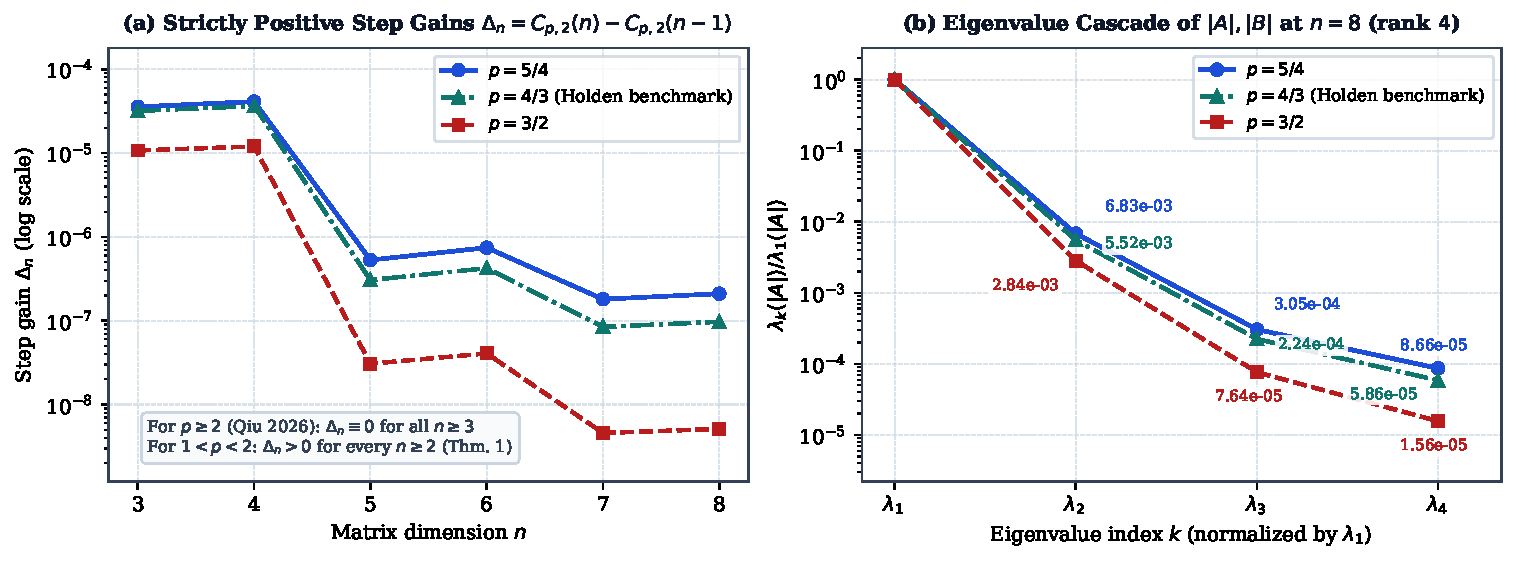
\includegraphics[width=\textwidth]{fig1_staircase_cascade.pdf}
  \vspace{-6pt}
  \caption{\small \emph{Left (a):} Strictly positive dimensional step gains $\Delta_n = C_{p,2}(n) - C_{p,2}(n-1)$ across $n = 3,\dots,8$ for $p = 5/4$ (blue circles), $p = 4/3$ (teal triangles, Holden's benchmark exponent~\cite{Holden2026}), and $p = 3/2$ (red squares), contrasting with $p \ge 2$ where $\Delta_n \equiv 0$ for all $n \ge 3$~\cite{Qiu2026}. Notice the paired odd/even plateau structure arising from the alternating rank growth $(1,1)\to(2,1)\to(2,2)\to\cdots$. \emph{Right (b):} Normalized nonzero eigenvalues of $|A|$ (equal to those of $|B|$) at $n = 8$ (rank~$4$), showing rapid geometric decay.}
  \label{fig:cascade}
\end{figure}

\begin{table}[H]
\centering
\caption{\small High-precision staircase $C_{3/2,2}(n)$ for $p = 3/2, m = 2$ (Tang--Zhang formula: $1.0346539519$).}
\vspace{3pt}
\footnotesize
\begin{tabular}{@{}c c l l l@{}}
\toprule
\textbf{Dim $n$} & \textbf{Ranks ($\rank A, \rank B$)} & \textbf{$C_{3/2,2}(n)$} & \textbf{Step gain $\Delta_n$} & \textbf{Normalized nonzero eigenvalues of $|A|$} \\
\midrule
2 & $(1,1)$ & $1.03641435733341^*$ & $+3.641\times 10^{-2}$ & $[1.00]$ \\
3 & $(2,1)$ & $1.03642509117441$   & $+1.073\times 10^{-5}$ & $[1.00,\; 2.47\times 10^{-3}]$ \\
4 & $(2,2)$ & $1.03643708623764$   & $+1.200\times 10^{-5}$ & $[1.00,\; 2.79\times 10^{-3}]$ \\
5 & $(3,2)$ & $1.03643711693849$   & $+3.070\times 10^{-8}$ & $[1.00,\; 2.81\times 10^{-3},\; 5.46\times 10^{-5}]$ \\
6 & $(3,3)$ & $1.03643715767551$   & $+4.074\times 10^{-8}$ & $[1.00,\; 2.84\times 10^{-3},\; 7.63\times 10^{-5}]$ \\
7 & $(4,3)$ & $1.03643716225772$   & $+4.582\times 10^{-9}$ & $[1.00,\; 2.84\times 10^{-3},\; 7.63\times 10^{-5},\; 1.38\times 10^{-5}]$ \\
8 & $(4,4)$ & $1.03643716738222$   & $+5.125\times 10^{-9}$ & $[1.00,\; 2.84\times 10^{-3},\; 7.64\times 10^{-5},\; 1.56\times 10^{-5}]$ \\
\bottomrule
\end{tabular}
\label{tab:p32}
\end{table}

\begin{table}[H]
\centering
\caption{\small High-precision staircase $C_{4/3,2}(n)$ for $p = 4/3, m = 2$ (Tang--Zhang: $1.0137583436$; Holden certified enclosure~\cite{Holden2026}: $1.018371575 < C_{4/3,2}(\infty) \le (861/800)^{1/4} \approx 1.0185404735$).}
\vspace{3pt}
\footnotesize
\begin{tabular}{@{}c c l l l@{}}
\toprule
\textbf{Dim $n$} & \textbf{Ranks ($\rank A, \rank B$)} & \textbf{$C_{4/3,2}(n)$} & \textbf{Step gain $\Delta_n$} & \textbf{Normalized nonzero eigenvalues of $|A|$} \\
\midrule
2 & $(1,1)$ & $1.01830237543067^*$ & $+1.830\times 10^{-2}$ & $[1.00]$ \\
3 & $(2,1)$ & $1.01833420141557$   & $+3.183\times 10^{-5}$ & $[1.00,\; 4.38\times 10^{-3}]$ \\
4 & $(2,2)$ & $1.01837064274052$   & $+3.644\times 10^{-5}$ & $[1.00,\; 5.19\times 10^{-3}]$ \\
5 & $(3,2)$ & $1.01837094872573$   & $+3.060\times 10^{-7}$ & $[1.00,\; 5.30\times 10^{-3},\; 1.43\times 10^{-4}]$ \\
6 & $(3,3)$ & $1.01837137193796$   & $+4.232\times 10^{-7}$ & $[1.00,\; 5.48\times 10^{-3},\; 2.22\times 10^{-4}]$ \\
7 & $(4,3)$ & $1.01837145645530$   & $+8.452\times 10^{-8}$ & $[1.00,\; 5.50\times 10^{-3},\; 2.23\times 10^{-4},\; 4.93\times 10^{-5}]$ \\
8 & $(4,4)$ & $1.01837155358673$   & $+9.713\times 10^{-8}$ & $[1.00,\; 5.52\times 10^{-3},\; 2.24\times 10^{-4},\; 5.86\times 10^{-5}]$ \\
\bottomrule
\end{tabular}
\label{tab:p43}
\end{table}

\begin{table}[H]
\centering
\caption{\small High-precision staircase $C_{5/4,2}(n)$ for $p = 5/4, m = 2$ (Tang--Zhang formula: $1.0057587726$).}
\vspace{3pt}
\footnotesize
\begin{tabular}{@{}c c l l l@{}}
\toprule
\textbf{Dim $n$} & \textbf{Ranks ($\rank A, \rank B$)} & \textbf{$C_{5/4,2}(n)$} & \textbf{Step gain $\Delta_n$} & \textbf{Normalized nonzero eigenvalues of $|A|$} \\
\midrule
2 & $(1,1)$ & $1.01098753445242^*$ & $+1.099\times 10^{-2}$ & $[1.00]$ \\
3 & $(2,1)$ & $1.01102311501737$   & $+3.558\times 10^{-5}$ & $[1.00,\; 5.11\times 10^{-3}]$ \\
4 & $(2,2)$ & $1.01106425559437$   & $+4.114\times 10^{-5}$ & $[1.00,\; 6.21\times 10^{-3}]$ \\
5 & $(3,2)$ & $1.01106478536413$   & $+5.298\times 10^{-7}$ & $[1.00,\; 6.41\times 10^{-3},\; 1.83\times 10^{-4}]$ \\
6 & $(3,3)$ & $1.01106552894231$   & $+7.436\times 10^{-7}$ & $[1.00,\; 6.74\times 10^{-3},\; 3.00\times 10^{-4}]$ \\
7 & $(4,3)$ & $1.01106570953544$   & $+1.806\times 10^{-7}$ & $[1.00,\; 6.78\times 10^{-3},\; 3.03\times 10^{-4},\; 7.09\times 10^{-5}]$ \\
8 & $(4,4)$ & $1.01106591970515$   & $+2.102\times 10^{-7}$ & $[1.00,\; 6.83\times 10^{-3},\; 3.05\times 10^{-4},\; 8.66\times 10^{-5}]$ \\
\bottomrule
\end{tabular}
\label{tab:p54}
\end{table}

\noindent{\footnotesize\textsuperscript{*}Exact analytical values from Theorem~3. For $m = 3$ at $p = 3/2$, Theorem~3 proves $C_{3/2,3}(2) = C_{3/2,2}(2) \approx 1.036414357333$, while exact-gradient optimization confirms strict dimensional growth across $n = 2, 3, 4, 5$: $1.036414357333 < 1.063086305441 < 1.063090693728 < 1.063095357075$ (compare Tang--Zhang $C_{3/2,3}^{\TZ} \approx 1.0607584802$). At $p = 4/3$, Holden's certified lower bound $1.018371575$~\cite{Holden2026} strictly exceeds our exact $2\times 2$ barrier $C_{4/3,2}(2) \approx 1.0183023754$ (by $+6.92\times 10^{-5}$) and lies just above our $n = 10$ optimization value $1.0183715701$, consistent with Holden's higher-order cyclic block construction and our Theorem~1.}

\subsection{Independent Exact-Rational, Symbolic, and 10-Line Verification}

All analytical identities and numerical claims were independently verified by two reproducible scripts bundled with this whitepaper:
\begin{itemize}[leftmargin=1.5em,itemsep=2pt]
  \item \textbf{Zero-float exact rational certificates (\texttt{verify\_exact\_certificates.py}):} Using only Python's standard library (\texttt{fractions}, \texttt{math.isqrt}), all three witnesses in Theorem~4 are certified with Weyl perturbation radii $\epsilon_H < 1.5\times 10^{-39}$ and strictly positive certified gaps in integer powers ($+8.70\times 10^{-6}$ in 6th powers at $p = 3/2$; $+4.62\times 10^{-5}$ in 4th powers at $p = 4/3$; $+1.32\times 10^{-4}$ in 10th powers at $p = 5/4$).
  \item \textbf{Symbolic and 105-digit audit (\texttt{verify\_all\_math.py}):} SymPy verifies all derivative factorizations, palindromic reductions, and Sturm uniqueness for Theorem~3 across $p \in \{3/2, 4/3, 5/4\}$. Across $5{,}000$ random complex PSD matrices (half rank-deficient), Lemma~4(a) holds with $\max(\mathrm{LHS}-\mathrm{RHS}) = -1.36\times 10^{-9}$; the dual Cauchy--Schwarz inequality of Theorem~3 holds across $5{,}000$ random complex tuples ($\max = -1.29\times 10^{-1}$); Lemma~2 strictly increases $\|S\|_p$ on $100/100$ random rank-deficient tuples in 105-digit \texttt{mpmath} arithmetic; and Lemma~4(b)'s explicit $\varepsilon_*$ strictly lifts $n = 2 \to 3$ with actual gain exceeding the certified lower bound across $p \in \{5/4, 4/3, 3/2, 7/4\}$.
\end{itemize}

\clearpage
The following self-contained 10-line NumPy snippet reproduces Theorem~4(1) in under one second:
\begin{tcolorbox}[codebox]
\begin{lstlisting}
import numpy as np
p = 1.5
sp = lambda M: np.sum(np.linalg.svd(M, compute_uv=False)**p)**(1/p)
ab = lambda M: (lambda _, s, vt: (vt.T * s) @ vt)(*np.linalg.svd(M, full_matrices=False))
A = np.array([[49., 62., -1.], [11., 14., 0.], [0., 0., 0.]])
B = np.array([[81.,  0.,  0.], [ 0.,  0., 0.], [0., 0., 0.]])
C2 = ((107 + 51*np.sqrt(17)) / 256)**(1/6)  # exact 2x2 supremum (Theorem 3)
ratio = sp(A + B) / sp(ab(A) + ab(B))
print(f"2x2 supremum = {C2:.15f}\n3x3 integer  = {ratio:.15f}\ngap = {ratio - C2:+.3e}")
\end{lstlisting}
\end{tcolorbox}
\vspace{-2pt}
{\ttfamily\footnotesize\color{ink} Output: 2x2 supremum = 1.036414357333407 \;|\; 3x3 integer = 1.036415570430780 \;|\; gap = +1.213e-06.}

\section{Remaining Open Questions for MI-20}

While Theorems~1--4 completely settle the finite-dimensional and finite-rank attainment structure of Problem~MI-20—ruling out every finite-dimensional and every finite-rank candidate extremizer—determining the exact constant $C_p(m)$ remains open through two central infinite-dimensional questions:
\begin{enumerate}[leftmargin=1.6em,itemsep=3pt]
  \item \textbf{Existence of an infinite-rank extremizer.} For $1 < p < 2$ and $m \ge 2$, does there exist a tuple of infinite-rank compact operators $(A_1,\dots,A_m) \in (\Sp(\ell^2))^m$ attaining $C_{p,m}(\infty)$, or is even the Hilbert-space supremum unattained? In particular, does the observed geometric eigenvalue cascade in Figure~\ref{fig:cascade}(b) converge to an explicit infinite-rank extremizer in $\Sp(\ell^2)$?
  \item \textbf{Analytical evaluation of $C_{p,m}(\infty)$.} Can the limiting constant (e.g., $C_{3/2,2}(\infty) \approx 1.03643717\dots$, $C_{4/3,2}(\infty) \in [1.018371575, 1.0185404735]$, $C_{5/4,2}(\infty) \approx 1.011066\dots$) be evaluated explicitly via Holden's positive power-system equations~\cite{Holden2026} on $\ell^2$ or an operator-theoretic Euler--Lagrange characterization?
\end{enumerate}

\begin{thebibliography}{9}
\small
\bibitem{Lee2010}
E.-Y. Lee, \emph{Rotfel'd type inequalities for norms}, Linear Algebra and its Applications \textbf{433}(3) (2010), 580--584.

\bibitem{Lee2011}
E.-Y. Lee, \emph{Extension of Rotfel'd theorem}, Linear Algebra and its Applications \textbf{435}(4) (2011), 735--741.

\bibitem{LinZhang2022}
J. Lin and Y. Zhang, \emph{A proof of Lee's conjecture on the sum of absolute values of matrices}, Journal of Mathematical Analysis and Applications \textbf{516} (2022), 126542.

\bibitem{TangZhang2026}
Q. Tang and S. Zhang, \emph{Generalizing Lee's conjecture on the sum of absolute values of matrices}, Linear Algebra and its Applications \textbf{731} (2026), 196--204; arXiv:2510.16846.

\bibitem{Zeng2026}
Z. Zeng, H. Liu, and K. Ratnavelu, \emph{A counterexample to the Tang--Zhang Schatten norm conjecture and sharp positive results}, arXiv:2608.15558 (August 2026).

\bibitem{Qiu2026}
H. Qiu, \emph{Sharp quasi-reverse Minkowski inequality for Schatten norms}, arXiv:2608.17565v2 (August 2026).

\bibitem{Li2026}
X. Li, \emph{Sharp concave-function transfer for Lee-type Schatten norm inequalities}, arXiv:2608.25989v1 (August 2026).

\bibitem{Holden2026}
S. Holden, \emph{MI-20, Round Four: An Exact Universal Bound and a Positive Power-System Reduction}, partial-result report archived in \emph{Open Problems in Numerical Linear Algebra} (\nolinkurl{references/holden-continuations-2026-09-13/MI-20/report.pdf}), September 2026.

\bibitem{OpenProblemsNLA}
A. Townsend et al., \emph{Open Problems in Numerical Linear Algebra (OpenProblemsInNLA)}, Problem MI-20: \emph{Sharp subquadratic Lee constants for sums of matrices}, \url{https://github.com/ajt60gaibb/OpenProblemsInNLA} (2026).
\end{thebibliography}

\end{document}
